\section{Versuchsaufbau/-durchführung}
Eine schematische Darstellung des Aufbaus zur Aktivierung der verwendeten Proben befindet sich in Abbildung \ref{fig: neutronenquelle}.
Die beiden Isotope \ce{^9 Be} und \ce{^226 Ra} sind hierbei innerhalb eines Stahlbehälters von Paraffin umgeben, in das durch Bohrungen
die zu aktivierenden Proben eingeführt werden können.\\
Im Anschluss werden die Proben in den Aufbau nach Abbildung \ref{fig: aufbau} integriert.
Zum Nachweis der $\beta$- bzw. $\gamma$-Strahlung wird ein Geiger-Müller-Zählrohr verwendet, dessen elektrische Signale
mittels eines Verstärkers erhöht werden. Ein Zählwerk registriert die Anzahl elektrischer Impulse innerhalb eines einstellbaren
Zeitintervalls $\Delta t$. Da das Gerät über zwei Anzeigen verfügt, zwischen denen nach Ablauf der Zeit $\Delta t$ automatisch gewechselt
wird, kann kontinuierlich gemessen werden. \\
Um den Nulleffekt für anschließende Messungen zu quantifizieren, wird zunächst
über einen Zeitraum von $\SI{900}{\second}$ ohne radioaktive Probe gemessen. Der Wert für die Nullrate in Formel \eqref{eq: nullrate}
ergibt sich dann, unter der Annahme einer etwa konstanten Nullrate, gemäß
\begin{equation}
  N\ua{0,\Delta t} = \frac{N\ua{0, \Delta t = \SI{900}{\second}}}{ \SI{900}{\second}} \Delta t.
\end{equation}
Für Indium wird über einen Zeitraum von $\SI{60}{\minute}$ im Zeitintervall $\Delta t = \SI{240}{\second}$ gemessen,
für Rhodium innerhalb von $\SI{12}{\minute}$ mit $\Delta t = \SI{15}{\second}$.
\begin{figure}
  \centering
  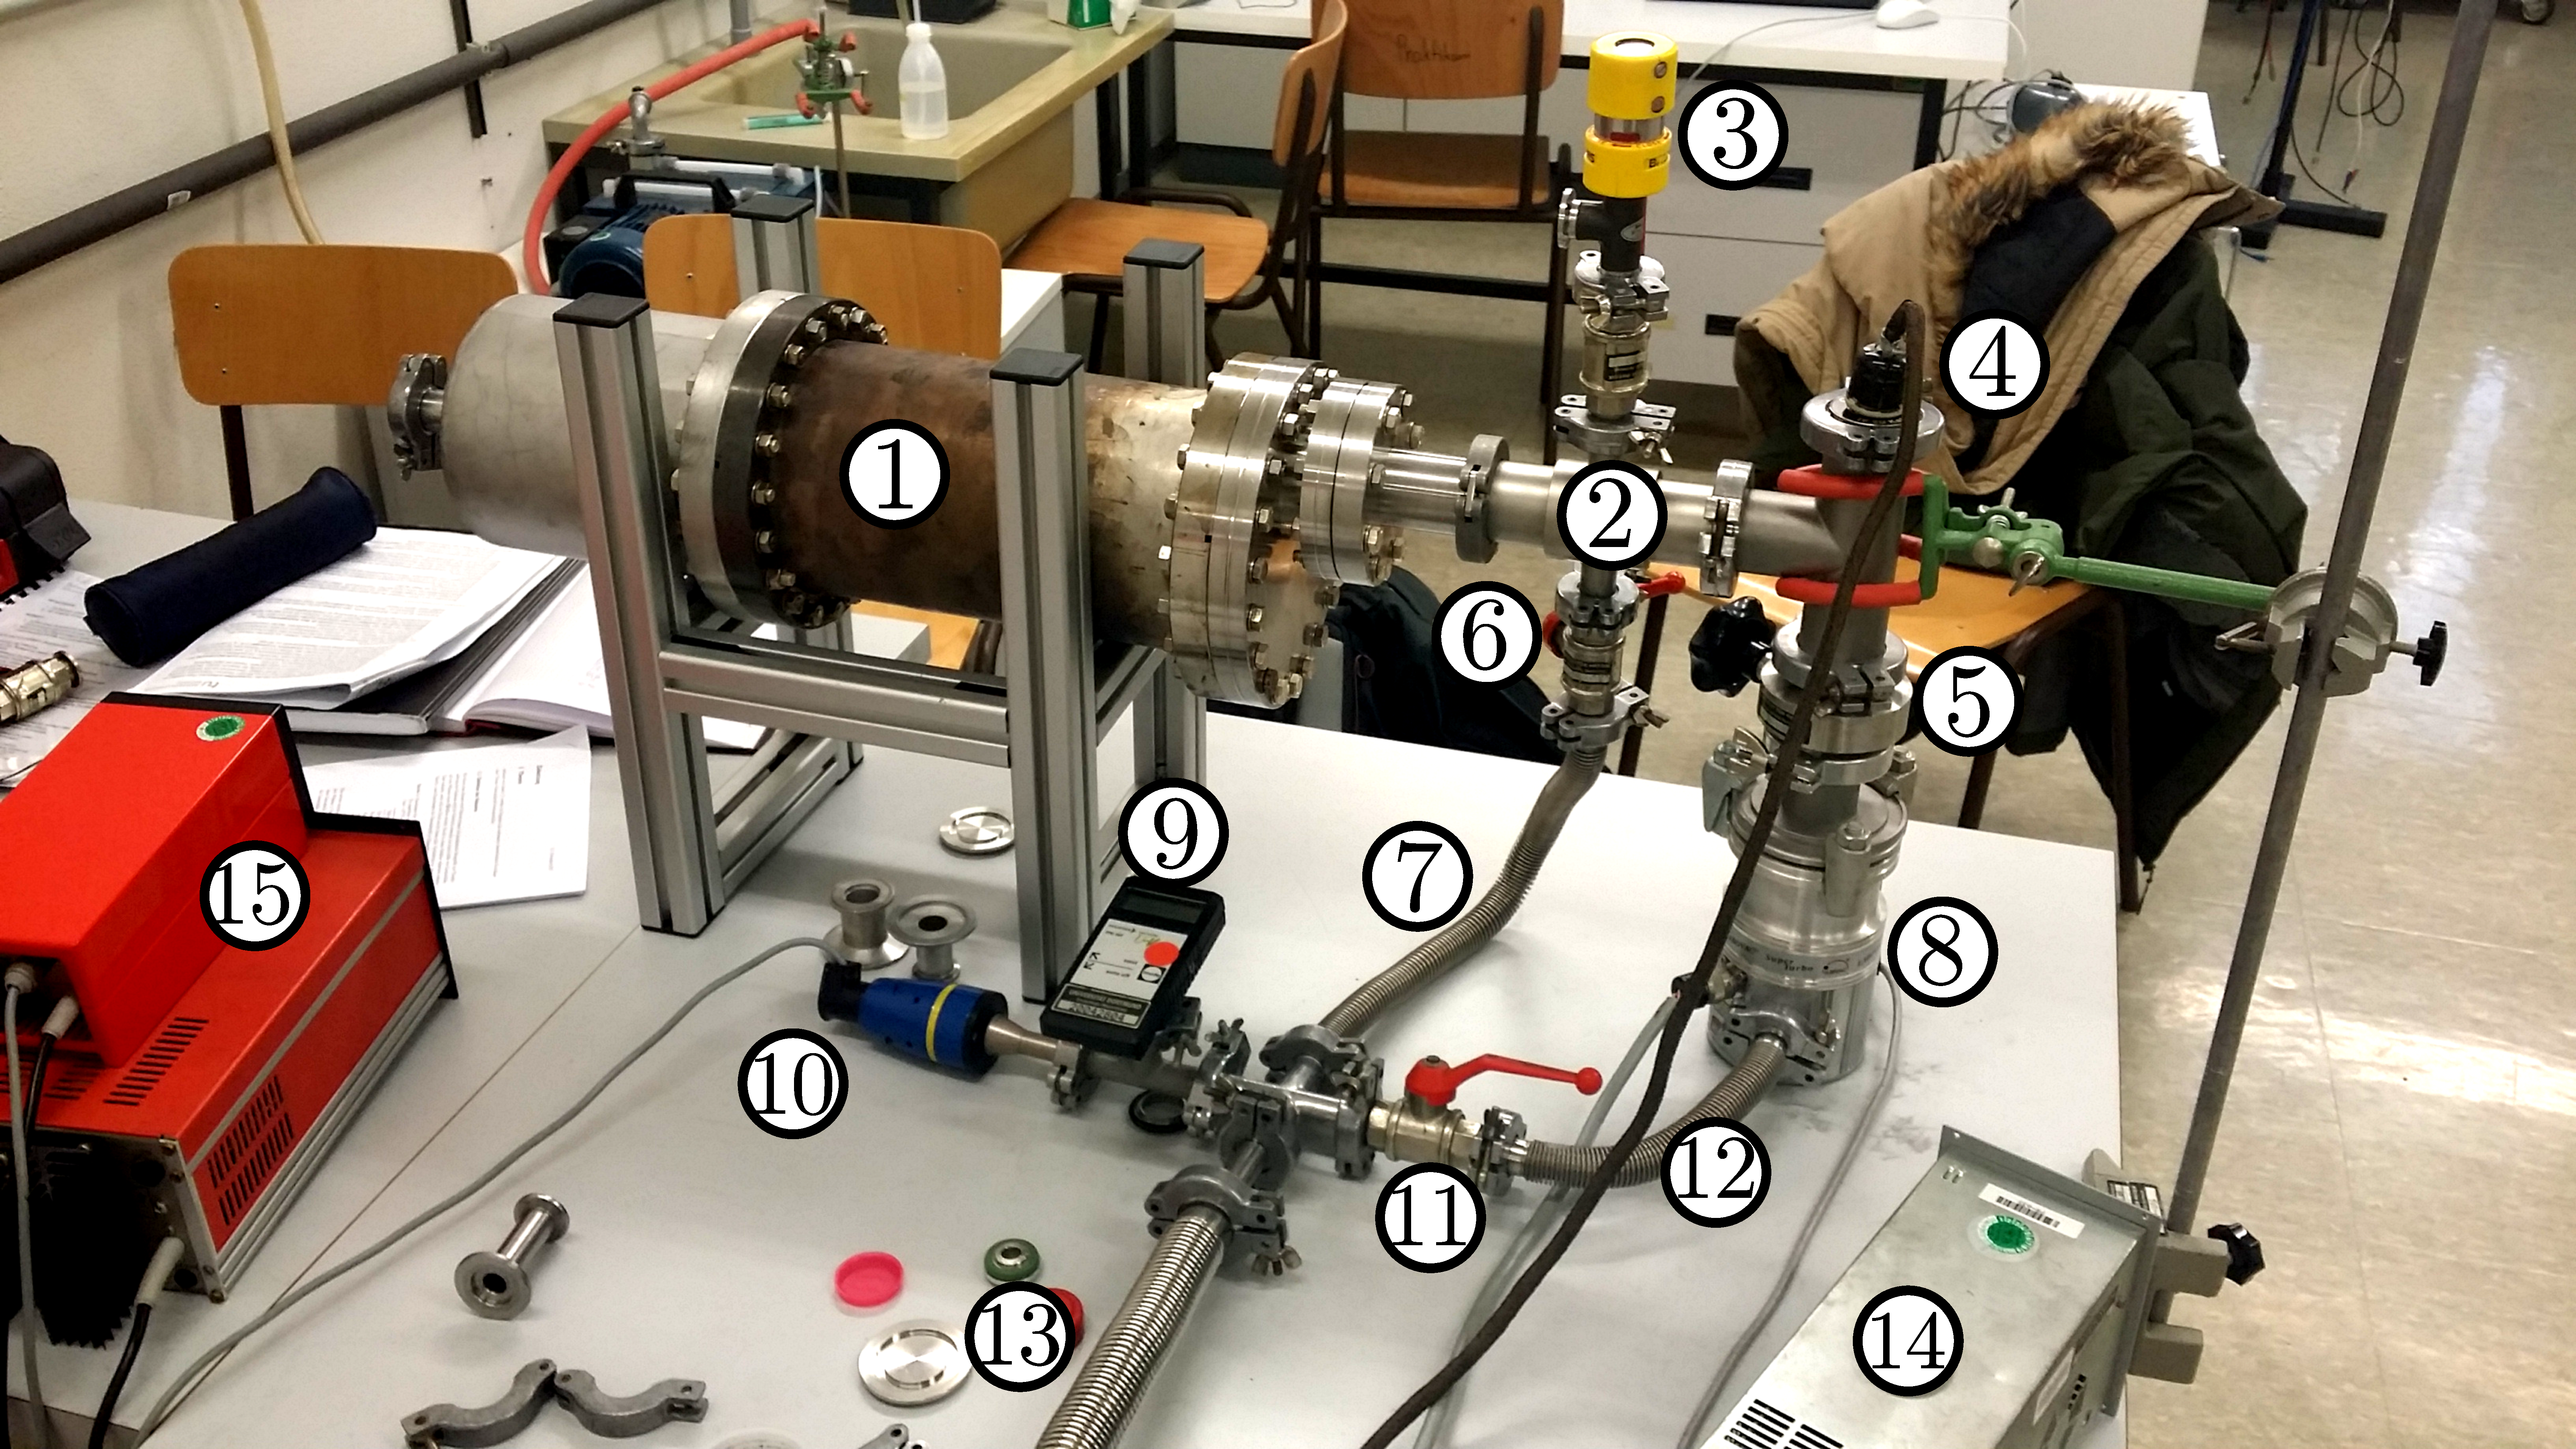
\includegraphics[width=0.9\textwidth]{pics/aufbau.png}
  \caption{Schematische Darstellung des Aufbaus zur Aktivierung der Proben \cite{anleitung702}(bearbeitet).}
  \label{fig: neutronenquelle}
  \end{figure}
\begin{figure}
\centering
\includegraphics[width=0.9\textwidth]{pics/aufbau_2.png}
\caption{Aufbau zur experimentellen Bestimmung der Halbwertszeit \cite{anleitung702}.}
\label{fig: aufbau}
\end{figure}
